\chapter{Rezultaty}
\section{Dobór parametrów algorytmu}
\begin{itemize}
\item tabelki z wyselekcjonowanymi parametrami, takie jak w excelu
%\item wykres dla Schaffer1 bestfitness_calych_scenariuszy_Schaffer1 
%\item fitness_etapow_scenariuszymutDefault_Schaffer1
%\item fitness_etapow_scenariuszymutGauss_Schaffer1
\end{itemize}

\begin{table}[hb]
\label{tab:selekcja_Schaffer_czasy}
\caption{Czasy i najlepsze rozwiązanie znalezione w trakcie selekcji parametrów algorytmów dla funkcji Schaffer nr 2}
\begin{center}
\begin{tabular}{|c|c|c|c|c|}
	\hline
	Algorytm & Mutacja & Najlepsze rozwiązanie & Czas selekcji [s] & Scenariusz \\
	\hline
	Memetyczny & \emph{mutDefault} & 0.03788 & 540.74 & $[1-2-3,\; 4-5-6]$\\
	Memetyczny & \emph{mutGauss} & 0.02769 & 584.67 & $[1-2-3,\; 4-5-6]$ \\
	Genetyczny & \emph{mutDefault} & 0.06609 & 171.79 & - \\
	Genetyczny & \emph{mutGauss} & 0.04549 & 186.90 & - \\
	PSO	& - & 0.09882 & 282.22 & -\\

	\hline
	\end{tabular}
\end{center}
\end{table}

\begin{table}[hb]
\label{tab:selekcja_Schaffer_parametry}
\caption{Dobrane wartości parametrów algorytmów dla funkcji Schaffer nr 2}
\begin{center}
\begin{tabular}{|c|c|c|c|c|c|c|c|}
	\hline
	Algorytm & Mutacja & $p_{mut}$ & $p_{cross}$ & $r_{pop}$ & $p_{opt}$ & $p_{sel}$ & Operator\\
	\hline
	Memetyczny & \emph{mutDefault} & 0.5 & 0.9 & 100 & 0.8 & 1.0 & \emph{L-BFGS-B} \\
	Memetyczny & \emph{mutGauss}  & 0.7 & 0.9 & 100 & 1.0 & 0.6 & \emph{L-BFGS-B} \\
	Genetyczny & \emph{mutDefault} & 0.6 & 0.9 & 100 & - & - & - \\
	Genetyczny & \emph{mutGauss}  & 0.5 & 1.0 & 100 & - & - & - \\
	\hline
	\end{tabular}

\begin{tabular}{|c|c|c|c|c|}
	\hline
	Algorytm & $\phi_1$ & $\phi_2$ & $w$ & $r_{pop}$ \\
	\hline
	PSO & 1.6 & 2.5 & 1.0 & 100 \\
	\hline
\end{tabular}
\end{center}
\end{table}
              
\begin{table}[hb]
\label{tab:selekcja_Paviani_czasy}
\caption{Czasy i najlepsze rozwiązanie znalezione w trakcie selekcji parametrów algorytmów dla funkcji Paviani}
\begin{center}
\begin{tabular}{|c|c|c|c|c|}
	\hline
	Algorytm & Mutacja & Najlepsze rozwiązanie & Czas selekcji [s] & Scenariusz \\
	\hline
	Memetyczny & \emph{mutDefault} & -45.77847 & 849.00 & $[4-5-6,\; 1-2-3]$\\
	Memetyczny & \emph{mutGauss} & -45.77847 & 841.99 & $[4-5-6,\; 1-2-3]$ \\
	Genetyczny & \emph{mutDefault} & -24.71857 & 212.64 & - \\
	Genetyczny & \emph{mutGauss} & -23.36381 & 218.80 & - \\
	PSO	& - & -37.78442 & 412.75 & -\\

	\hline
	\end{tabular}
\end{center}
\end{table}

\begin{table}[hb]
\label{tab:selekcja_Paviani_parametry}
\caption{Dobrane wartości parametrów algorytmów dla funkcji Paviani}
\begin{center}
\begin{tabular}{|c|c|c|c|c|c|c|c|}
	\hline
	Algorytm & Mutacja & $p_{mut}$ & $p_{cross}$ & $r_{pop}$ & $p_{opt}$ & $p_{sel}$ & Operator\\
	\hline
	Memetyczny & \emph{mutDefault} & 0.5 & 0.7 & 100 & 1.0 & 1.0 & \emph{L-BFGS-B} \\
	Memetyczny & \emph{mutGauss}  & 0.8 & 0.9 & 100 & 1.0 & 0.9 & \emph{L-BFGS-B} \\
	Genetyczny & \emph{mutDefault} & 0.8 & 0.7 & 100 & - & - & - \\
	Genetyczny & \emph{mutGauss}  & 1.0 & 1.0 & 100 & - & - & - \\
	\hline
	\end{tabular}

\begin{tabular}{|c|c|c|c|c|}
	\hline
	Algorytm & $\phi_1$ & $\phi_2$ & $w$ & $r_{pop}$ \\
	\hline
	PSO & 1.0 & 3.1 & 0.8 & 100 \\
	\hline
\end{tabular}
\end{center}
\end{table}

\begin{table}[hb]
\label{tab:selekcja_Zeldasine_czasy}
\caption{Czasy i najlepsze rozwiązanie znalezione w trakcie selekcji parametrów algorytmów dla funkcji ZeldaSine10}
\begin{center}
\begin{tabular}{|c|c|c|c|c|}
	\hline
	Algorytm & Mutacja & Najlepsze rozwiązanie & Czas selekcji [s] & Scenariusz \\
	\hline
	Memetyczny & \emph{mutDefault} & -3.5 & 243.22 & $[4-5,\;3-6,\;1-2]$\\
	Memetyczny & \emph{mutGauss} & -3.5 & 190.31 & $[4-5,\;3-6,\;1-2]$ \\
	Genetyczny & \emph{mutDefault} & -1.69261 & 206.83 & - \\
	Genetyczny & \emph{mutGauss} & -1.81252 & 214.95 & - \\
	PSO	& - & -0.91760 & 36.15 & -\\

	\hline
	\end{tabular}
\end{center}
\end{table}

\begin{table}[hb]
\label{tab:selekcja_Zeldasine_parametry}
\caption{Dobrane wartości parametrów algorytmów dla funkcji ZeldaSine10}
\begin{center}
\begin{tabular}{|c|c|c|c|c|c|c|c|}
	\hline
	Algorytm & Mutacja & $p_{mut}$ & $p_{cross}$ & $r_{pop}$ & $p_{opt}$ & $p_{sel}$ & Operator\\
	\hline
	Memetyczny & \emph{mutDefault} & 0.7 & 1.0 & 100 & 0.6 & 0.6 & \emph{L-BFGS-B} \\
	Memetyczny & \emph{mutGauss}  & 0.9 & 1.0 & 50 & 1.0 & 0.6 & \emph{L-BFGS-B} \\
	Genetyczny & \emph{mutDefault} & 0.8 & 0.9 & 100 & - & - & - \\
	Genetyczny & \emph{mutGauss}  & 0.9 & 1 & 100 & - & - & - \\
	\hline
	\end{tabular}

\begin{tabular}{|c|c|c|c|c|}
	\hline
	Algorytm & $\phi_1$ & $\phi_2$ & $w$ & $r_{pop}$ \\
	\hline
	PSO & 1.6 & 2.5 & 1.0 & 100 \\
	\hline
\end{tabular}
\end{center}
\end{table}

\begin{figure} 
\centering
  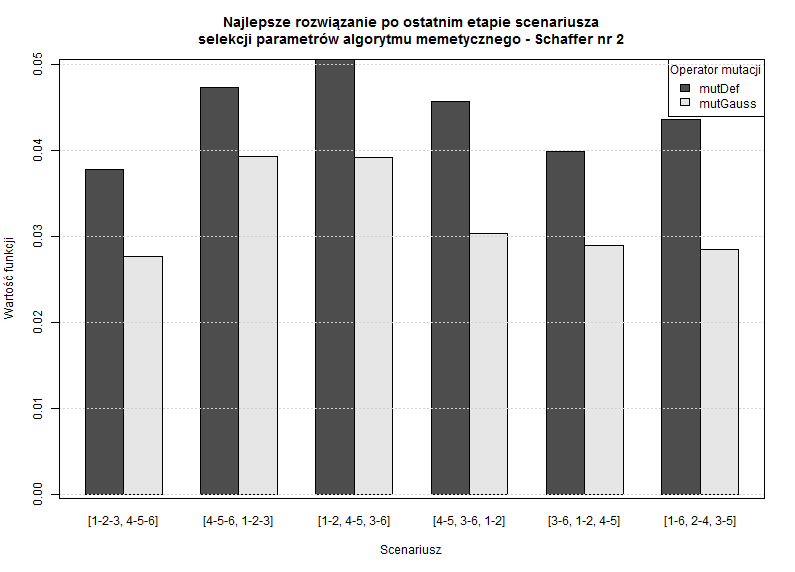
\includegraphics[width=\linewidth]{{img//roz04//parameterSelection//bestfitness_calych_scenariuszy_Schaffer1.png}}
\caption{Porównanie najlepszego rozwiązania dla różnych scenariuszy dla funkcji Schaffer nr 2}
\label{fig:parameter_selection_fitness_overall}
\end{figure}


\begin{figure} 
\centering
\begin{subfigure}{\textwidth}
  \centering
  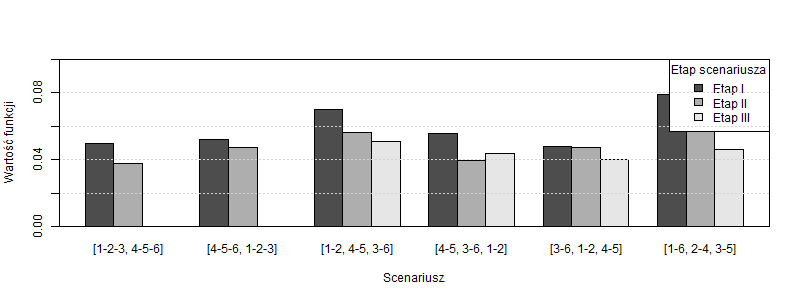
\includegraphics[width=\linewidth]{{img//roz04//parameterSelection//fitness_etapow_scenariuszymutDefault_Schaffer1.png}}
  \caption{\emph{mutDefault}}
  %\label{fig:sub1}
\end{subfigure}
\begin{subfigure}{\textwidth}
  \centering
  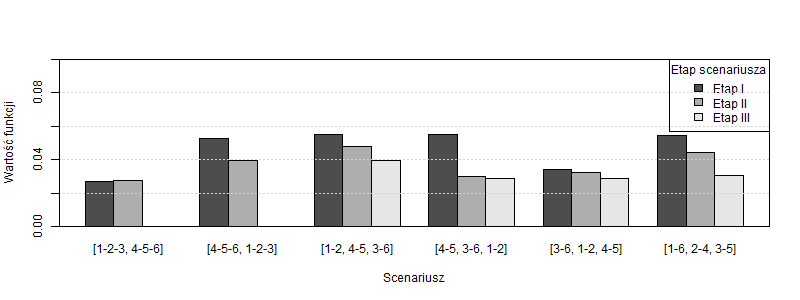
\includegraphics[width=\linewidth]{img//roz04//parameterSelection//fitness_etapow_scenariuszymutGauss_Schaffer1.png}
  \caption{\emph{mutGauss}}
  %\label{fig:sub2}
\end{subfigure}
\caption{Najlepsze znajdywane rozwiązanie kolejno w etapach selekcji dla funkcji Schaffer nr 2}
\label{fig:parameter_selection_fitness_in_phases}
\end{figure}
Pozostałe wykresy przedstawiono w dodatku...


\subsection{Algorytm memetyczny}
\begin{itemize}
\item porownanie skutecznosci scenariuszy
\item porownanie czasu wykonania scenariuszy
\end{itemize}
\subsection{Algorytm genetyczny i PSO}
\section{Miary efektywności}
\subsection{Kryterium nr 1 - najlepsze rozwiązanie}
\subsection{Kryterium nr 2 - szybkość osiągania rozwiązania}
\subsection{Kryterium nr 3 - powtarzalność skutecznej optymalizacji}
\subsection{Kryterium nr 4 - ogólna charakterystyka populacji}